%Settings for Bibliography Appendix
\renewcommand{\bibpreamble}{}
\renewcommand{\bibpostamble}{}
\renewcommand\bibfont{\normalfont\fontsize{8.58}{8}\selectfont}

%Content starts
\picturechapterlong{Curriculum vitae, List of publications, Acknowledgements}{Curriculum vitae, \\List of publications, \\Acknowledgements}{Chaptercovers/ch7.pdf} \label{ch-7}
{
	\begin{center}
		\vspace*{4cm}
		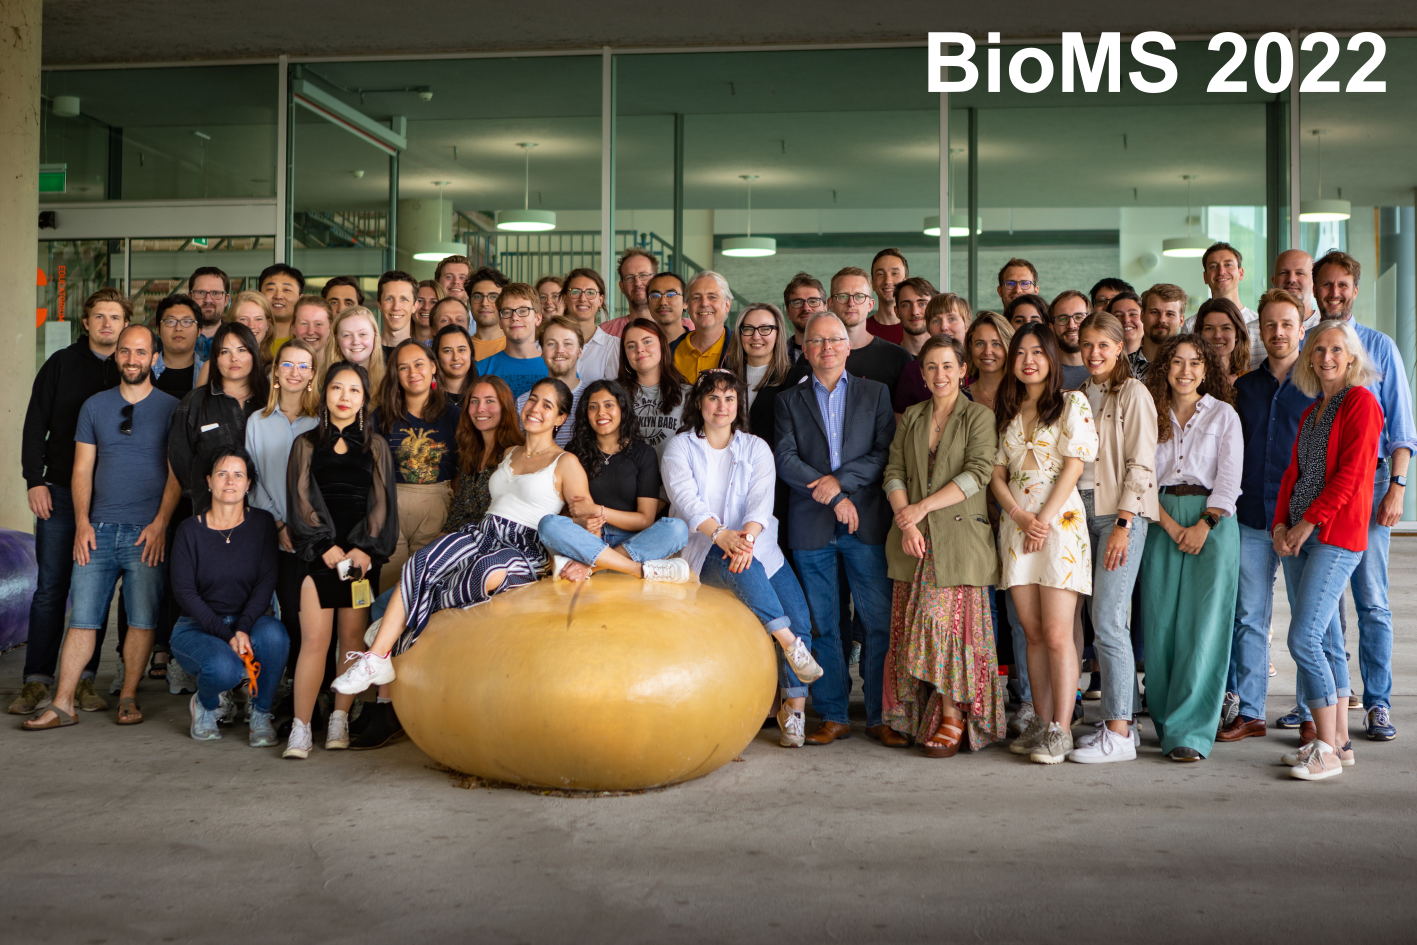
\includegraphics[]{Chapter.7/Figures/group2022.png}
		\vspace{0.25cm}
	\end{center}
}
\clearpage
\thumbforchapter
\section{Curriculum vitae}
I was born on the 11\textsuperscript{th} of September 1991 in Utrecht, the Netherlands. After finishing high school in 2012, I started my Bachelor studies in Pharmaceutical Sciences in Utrecht in 2012. During my bachelors I focussed on medicinal and organic chemistry, developing a strong interest in chemical interventions on the biological processes of our body. The completion of my studies was marked by writing my Bachelor thesis entitled “\emph{Explorative synthesis toward an asymmetrically protected entero-bactin derivative suitable for conjugation using CuAAC}”, which I conducted in the research group of Prof. dr. Roland Pieters (Utrecht University), but also by the realisation that I did not want to perform experiments, but rather focus my efforts on the computational front. In 2016, started my Master studies in drug innovation, with a bioinformatics course load. My first computational research project was at the Computational Structural Biology lab of Prof. Dr. Alexandre Bonvin, and involved protein-protein docking. Continuing along this line of structural biology, I then joined the biomolecular mass spectrometry group under the supervision of my current copromotor, Dr. Richard Scheltema, but now using proteomic crosslinking MS data. I truly found my passion in mass spectrometry. The simultaneous simplicity and versatility of "molecular scales" as my copromotor Richard so aptly puts it, being applied to yield rich data and achieve so many different goals continues to amaze me. I decided to stay with the group to write a research project, which ended up being the subject of my PhD under the supervision of Prof. dr. Albert Heck and Dr. Richard Scheltema in 2019, after a brief stint of travelling and work at a startup at the Delft University of Technology. Leveraging the computational skills I had acquired, we set out to achieve what then seemed like a herculean task, sequencing endogenous antibodies. However, as presented throughout this thesis, we managed to not only achieve this but pave the way towards a more generalizable workflow.
\clearpage
\section{List of publications}
\nocite{*}
\bibliographystyle{Stylesettings/pnasAllNames}
\patchcmd{\thebibliography}
{\clubpenalty 4000\widowpenalty 4000}
{\clubpenalties 1 10000 \widowpenalties 1 10000 }
{}{}
\bibliography{Chapter.7/mypublications.bib}
\clearpage
\section{Acknowledgements}

This Ph.D. thesis represents the culmination of an incredible journey, and I would like to express my heartfelt gratitude to the wonderful individuals who played crucial roles in its completion. Their unwavering support, expertise, and spirit have made this endeavor possible.

\textbf{Albert}, I am immensely grateful for your invaluable input. While our perspectives may not have always aligned, I have always felt assured knowing that I could rely on your insight and judgment. Your presence and knowledge have been a pillar of strength throughout this journey. Likewise, I extend my deepest appreciation to \textbf{Richard}. Your guidance in informatics and programming, as well as life and career advice, have been instrumental in shaping the trajectory of my Ph.D. To both of you, your wisdom, patience, and enthusiasm have not only expanded my knowledge but also inspired me to push the boundaries of scientific exploration.

I would like to acknowledge the collaborators who have contributed to all projects I was involved with. \textbf{Ron Heeren} and \textbf{Alexander Makarov}, your energy and wisdom were inspiring and elevated my research. \textbf{Wei Wu}, I want to thank you for including me in a captivating dive into the realms of genomics and immunopeptidomics. \textbf{Kelly}, I extend my heartfelt gratitude to you for making our collaboration a breeze. Your expertise and energy were instrumental in the completion of our profiling project.

My gratitude also goes to the Heck-lab IT-warriors, \textbf{Henk} and \textbf{Andris}, with whom I embarked on the collaborative journey of transforming and maintaining our core libraries. Your technical prowess and ability to appreciate even the lamest of coding jokes have made this process not only productive but even enjoyable. \textbf{Oleg}, \textbf{Pascal}, \textbf{Gadi}, and \textbf{Barbara}, I want to express my appreciation for your warm reception and invaluable contributions to CrossID. Your insights and welcoming personalities played a significant role in persuading me to embark on this transformative Ph.D. journey.

A profound thanks goes to the entire \textbf{Ig taskforce}, in particular \textbf{Jeff}, \textbf{Max}, \textbf{Douwe}, \textbf{Albert}, \textbf{Joost}, and \textbf{Weiwei}. Without your tireless dedication and collective efforts, I would have found myself at a loss, not just because of the lack of data but also due to the absence of your expertise and support.

I cannot overlook the contributions of the unsung heroines of the Heck lab, \textbf{Mirjam} and \textbf{Corine}. \textbf{Mirjam}, your coffee and the accompanying chitchat provided much-needed moments of respite on those days that everything seemingly went wrong. \textbf{Corine}, I am indebted to you for your patience, assistance, and willingness to help with any difficulties I encountered. I, and probably the whole lab, would undoubtedly be adrift without you both.

\textbf{Sem}, your patience, intelligence, and most of all friendship have meant so much for the completion of this thesis. I don't think I could have wished for a better person to guide me into the peculiarities of top-down mass spectrometry, or on how to sniff pickles and drink vodka. Similarly, a very special thanks goes to \textbf{Johannes}, with \textbf{Morgane} by his side, for being my steadfast companion throughout these years. Your incredible kindness, support, and understanding have made this journey exceptionally memorable. If I were to identify a single source of positive energy, it would undeniably be you.

\textbf{Riccardo}, and \textbf{Douwe}, you have been more than just office mates; you have become cherished friends. I am grateful for the camaraderie we shared, the conversations that sparked new ideas, and the laughter that brightened even the most challenging days. \textbf{Douwe}, in particular, I must thank you for your endless patience and insightful input on software design. I have learned invaluable lessons from you and am continually surprised by your extraordinary abilities.

I would like to acknowledge the wonderful colleagues and friends who have enriched my journey, \textbf{Dario}, \textbf{Wouter}, \textbf{Tim}, \textbf{Fujia}, \textbf{Donna}, \textbf{Julia}, \textbf{Vojtec}, and \textbf{Laura}. Despite my preference for remote work, your warmth and camaraderie have created an inspiring and supportive environment that I am deeply grateful for.

A special mention is reserved for my loving girlfriend, \textbf{Annemiek}, without whom this milestone would not have been possible. Your support, love, and encouragement during the most challenging moments have meant the world to me. I love and appreciate you like no other, and the connection we share has gotten me through hardships which may otherwise have been even more impactful. You are an incredible person, and I am grateful every day that I get to share my life with you.

To my parents, \textbf{Tiny} and \textbf{Frits}, I am eternally grateful for the collaborative efforts that have propelled me this far. You are my biggest role models, and your love, belief in my abilities, and sacrifices have shaped me into the person I am today. Beyond that, I extend my thanks to my family — \textbf{Ineke} and \textbf{Isabelle} in particular — for their enduring interest, support, and confidence, which have provided immeasurable strength throughout this journey.

I would be remiss not to mention my roommates and closest friends, \textbf{Mark}, \textbf{Jamie}, and \textbf{Laurens}. Your friendship and presence during relaxing nights, vibrant parties and delicious barbecues are a gift and were an essential source of relaxation throughout these past years.

Lastly, a special mention goes to \textbf{Bas Dutilh}, my serendipitous neighbor, colleague, and mentor. Your words of advice (and tolerance of my youthful shenanigans) have left an indelible mark on my journey, and I am profoundly grateful for that.

To all those mentioned, and to those whose names may have inadvertently been omitted, please know that your contributions, whether big or small, have played an integral role in the completion of this Ph.D. thesis. Your support, expertise, friendship, and belief in me have made this journey unforgettable. Thank you from the depths of my heart.

\stopthumb
\blankpage